\newpage
\section{第 05 周}

\subsection{第 12 课 | 动态规划}

\subsubsection{脑图}

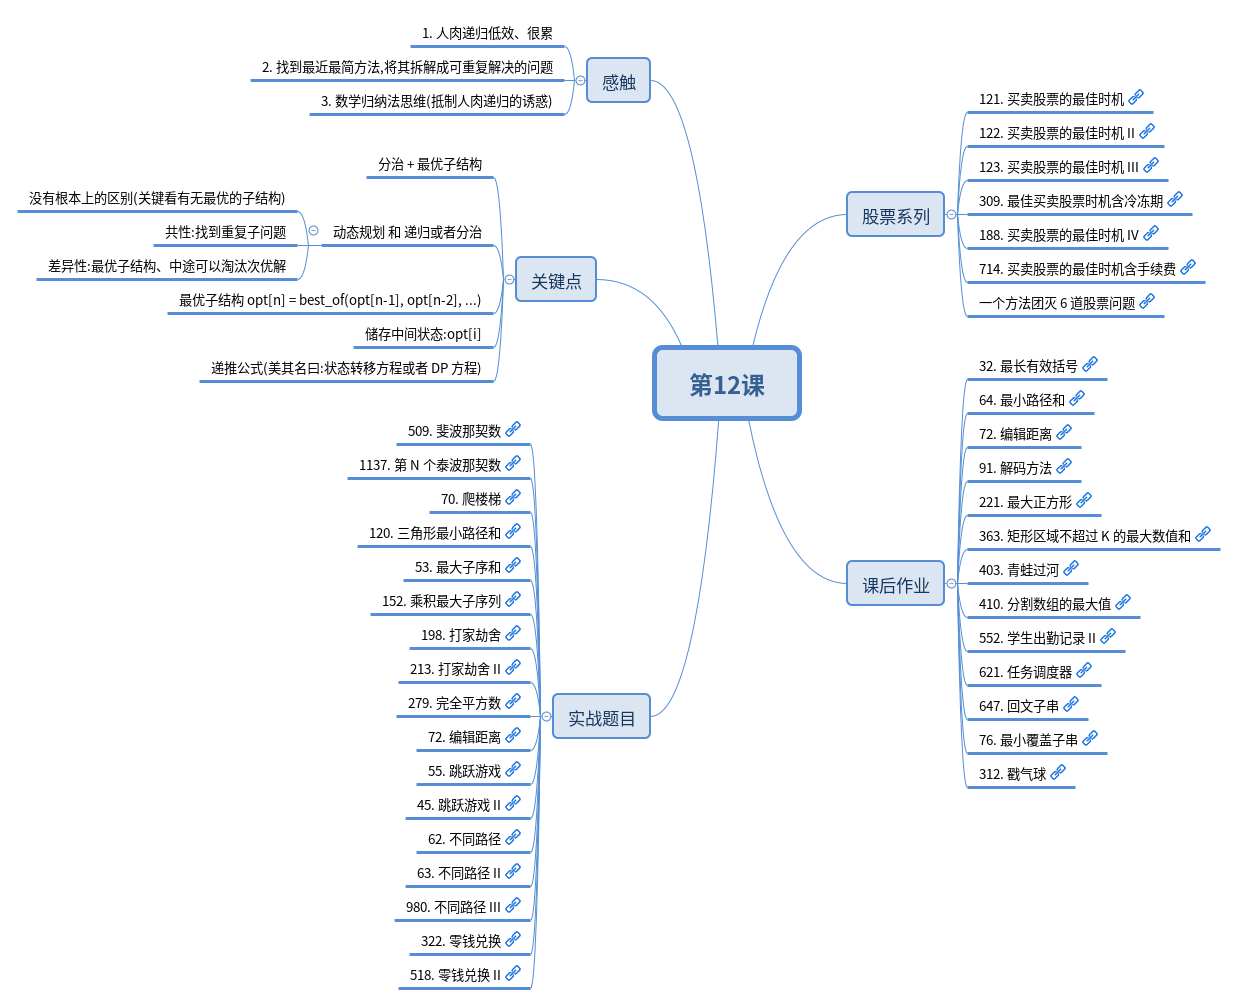
\includegraphics[width=170mm,height=160mm]{images/camp/第12课.png}

\subsubsection{题目}

\paragraph{实战题目}

\begin{itemize}
  \item \hyperref[leetcode:509]{509. 斐波那契数}
  \item \hyperref[leetcode:1137]{1137. 第 N 个泰波那契数}
  \item \hyperref[leetcode:70]{70. 爬楼梯}
  \item \hyperref[leetcode:120]{120. 三角形最小路径和}
  \item \hyperref[leetcode:53]{53. 最大子序和}
  \item \hyperref[leetcode:152]{152. 乘积最大子序列}
  \item \hyperref[leetcode:198]{198. 打家劫舍}
  \item \hyperref[leetcode:213]{213. 打家劫舍 II}
\end{itemize}

\paragraph{高级 DP 实战题目}

\begin{itemize}
  \item \hyperref[leetcode:279]{279. 完全平方数}
  \item \hyperref[leetcode:72]{72. 编辑距离}
  \item \hyperref[leetcode:55]{55. 跳跃游戏}
  \item \hyperref[leetcode:45]{45. 跳跃游戏 II}
  \item \hyperref[leetcode:62]{62. 不同路径}
  \item \hyperref[leetcode:63]{63. 不同路径 II}
  \item \hyperref[leetcode:980]{980. 不同路径 III}
  \item \hyperref[leetcode:322]{322. 零钱兑换}
  \item \hyperref[leetcode:518]{518. 零钱兑换 II}
\end{itemize}

\paragraph{股票系列题目}

\begin{itemize}
  \item \hyperref[leetcode:121]{121. 买卖股票的最佳时机}
  \item \hyperref[leetcode:122]{122. 买卖股票的最佳时机 II}
  \item \hyperref[leetcode:123]{123. 买卖股票的最佳时机 III}
  \item \hyperref[leetcode:309]{309. 最佳买卖股票时机含冷冻期}
  \item \hyperref[leetcode:188]{188. 买卖股票的最佳时机 IV}
  \item \hyperref[leetcode:714]{714. 买卖股票的最佳时机含手续费}
  \item \href{https://leetcode-cn.com/problems/best-time-to-buy-and-sell-stock/solution/yi-ge-fang-fa-tuan-mie-6-dao-gu-piao-wen-ti-by-l-3/}{一个方法团灭 6 道股票问题}
\end{itemize}

\paragraph{课后作业}

\begin{itemize}
  \item \hyperref[leetcode:32]{32. 最长有效括号}
  \item \hyperref[leetcode:64]{64. 最小路径和}
  \item \hyperref[leetcode:72]{72. 编辑距离}
  \item \hyperref[leetcode:91]{91. 解码方法}
  \item \hyperref[leetcode:221]{221. 最大正方形}
  \item \hyperref[leetcode:363]{363. 矩形区域不超过 K 的最大数值和}
  \item \hyperref[leetcode:403]{403. 青蛙过河}
  \item \hyperref[leetcode:410]{410. 分割数组的最大值}
  \item \hyperref[leetcode:552]{552. 学生出勤记录 II}
  \item \hyperref[leetcode:621]{621. 任务调度器}
  \item \hyperref[leetcode:647]{647. 回文子串}
  \item \hyperref[leetcode:76]{76. 最小覆盖子串}
  \item \hyperref[leetcode:312]{312. 戳气球}
\end{itemize}


\subsection{学习总结}

这周学习了动态规划,这个还是挺难的。

动态规划关键点:

1. 最优子结构 opt[n] = best_of(opt[n-1], opt[n-2], ...)
2. 储存中间状态:opt[i]
3. 递推公式(美其名曰:状态转移方程或者 DP 方程)

感觉还是需要把基础的题目多刷几遍之后,才会更有感觉吧。
不然总觉得换个题目了就又不会了。
